\documentclass[aspectratio=169]{beamer}

% RPTU Theme setup
\usetheme[dunkelblau, frametotal=true, navigation=true, redhattext=false]{rptu}

\usepackage[english]{babel}
\usepackage{booktabs}
\usepackage{graphicx}
\graphicspath{{graphs/}}
\usepackage{xcolor}
\usepackage{tikz}
\usetikzlibrary{arrows.meta,positioning,fit}

% Meta Information
\title{Creating and benchmarking Learned DB Components using LLM}
\author{Preksha Shah}
\institute[RPTU]{\\[0.3cm]Master's Thesis \\ FB Informatik}
\date{\today}

\begin{document}
	
	% --- Slide 1: Title Page ---
	\begin{frame}[plain]
		\titlepage
	\end{frame}
	
	% --- Slide 2: Agenda ---
	\begin{frame}{Agenda}
		\tableofcontents
	\end{frame}
	
	% ==========================================
	\section{Motivation}
	
	% --- Slide 3: Merged (old 3+4) ---
	\begin{frame}{Why Learned Cardinality Estimation?}
		\begin{columns}[T]
			\column{0.48\textwidth}
			\textbf{The Problem}
			\begin{itemize}
				\item Bad cardinality estimates lead to catastrophic join orders
				\item Histograms and independence assumptions fail on correlated data
				\item Sampling is expensive at runtime and misses rare groups
			\end{itemize}
			
			\column{0.48\textwidth}
			\textbf{The Learned Approach}
			\begin{itemize}
				\item Deep learning models (MSCN) learn correlations directly from data
				\item Outperform traditional mathematical estimators
				\item \textbf{But:} Require massive labeled workloads (queries + true cardinalities)
				\item Obtaining labels via query execution is expensive and hard to scale
			\end{itemize}
		\end{columns}
	\end{frame}
	
	% ==========================================
	\section{Pipeline}
	
	% --- Slide 4: Pipeline ---
	\begin{frame}{Pipeline: From Schema to Trained Estimator}
		\vspace{-0.6cm}
		\begin{center}
		\resizebox{0.85\textwidth}{!}{%
		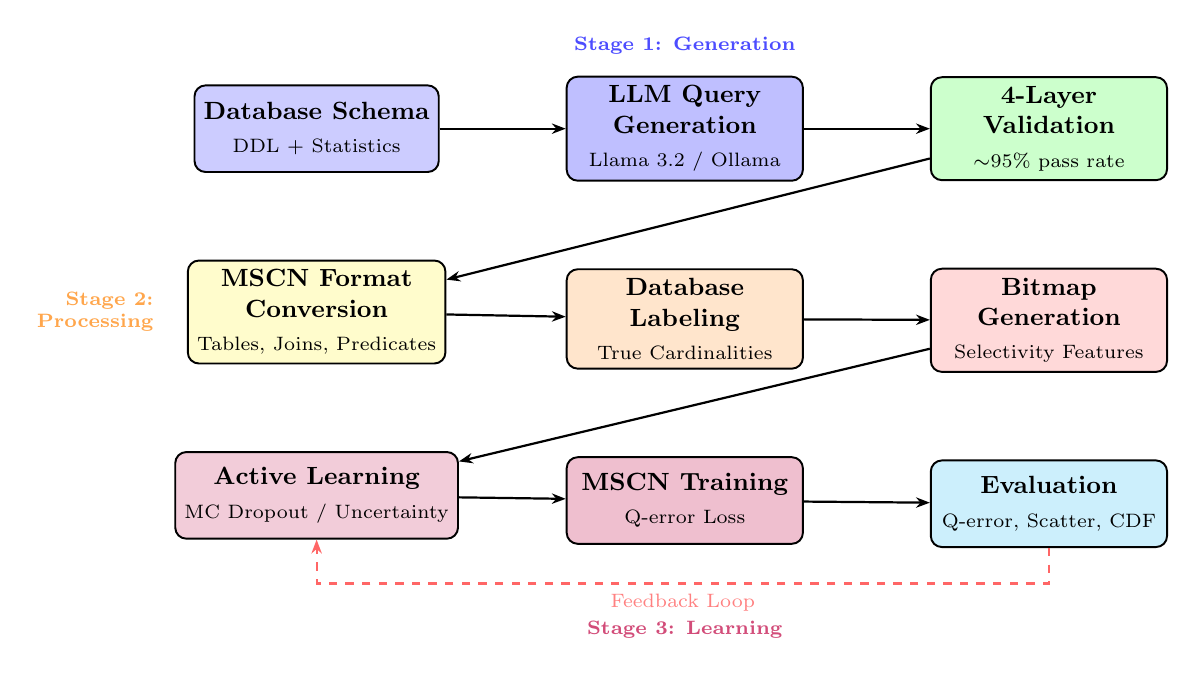
\begin{tikzpicture}[
		    node distance=1.1cm and 1.6cm,
		    block/.style={draw, rectangle, rounded corners=4pt, minimum width=3cm, minimum height=1.1cm, align=center, font=\small\bfseries, line width=0.7pt},
		    arr/.style={-{Stealth[length=5pt]}, thick},
		    darr/.style={-{Stealth[length=5pt]}, thick, dashed, red!60},
		]
		    % Row 1: Generation
		    \node [block, fill=blue!20] (schema) {Database Schema\\[1pt]{\scriptsize\normalfont DDL + Statistics}};
		    \node [block, fill=blue!25, right=of schema] (llm) {LLM Query\\Generation\\[1pt]{\scriptsize\normalfont Llama 3.2 / Ollama}};
		    \node [block, fill=green!20, right=of llm] (valid) {4-Layer\\Validation\\[1pt]{\scriptsize\normalfont $\sim$95\% pass rate}};
		    
		    % Row 2: Processing
		    \node [block, fill=yellow!20, below=of schema] (format) {MSCN Format\\Conversion\\[1pt]{\scriptsize\normalfont Tables, Joins, Predicates}};
		    \node [block, fill=orange!20, below=of llm] (label) {Database\\Labeling\\[1pt]{\scriptsize\normalfont True Cardinalities}};
		    \node [block, fill=red!15, below=of valid] (bitmap) {Bitmap\\Generation\\[1pt]{\scriptsize\normalfont Selectivity Features}};
		    
		    % Row 3: Learning
		    \node [block, fill=purple!20, below=of format] (al) {Active Learning\\[1pt]{\scriptsize\normalfont MC Dropout / Uncertainty}};
		    \node [block, fill=purple!25, below=of label] (train) {MSCN Training\\[1pt]{\scriptsize\normalfont Q-error Loss}};
		    \node [block, fill=cyan!20, below=of bitmap] (eval) {Evaluation\\[1pt]{\scriptsize\normalfont Q-error, Scatter, CDF}};
		    
		    % Row 1 arrows
		    \draw [arr] (schema) -- (llm);
		    \draw [arr] (llm) -- (valid);
		    
		    % Row 1 to Row 2
		    \draw [arr] (valid) -- (format);
		    \draw [arr] (format) -- (label);
		    \draw [arr] (label) -- (bitmap);
		    
		    % Row 2 to Row 3
		    \draw [arr] (bitmap) -- (al);
		    \draw [arr] (al) -- (train);
		    \draw [arr] (train) -- (eval);
		    
		    % Feedback loop
		    \draw [darr] (eval.south) -- ++(0,-0.45) -| (al.south) node[pos=0.25, below, font=\scriptsize, text=red!50] {Feedback Loop};
		    
		    % Stage labels
		    \node [above=0.15cm of llm, font=\scriptsize\bfseries, text=blue!70] {Stage 1: Generation};
		    \node [left=0.3cm of format, font=\scriptsize\bfseries, text=orange!70, align=right] {Stage 2:\\Processing};
		    \node [below=0.85cm of train, font=\scriptsize\bfseries, text=purple!70] {Stage 3: Learning};
		\end{tikzpicture}%
		}
		\end{center}
	\end{frame}
	
	% ==========================================
	\section{LLM Query Generation}
	
	% --- Slide 5: Merged (old 6+7) ---
	\begin{frame}{LLM-based Query Generation}
		\framesubtitle{Schema-aware prompting with diversity control}
		\small
		\begin{columns}[T]
			\column{0.48\textwidth}
			\textbf{Prompt Strategy:}
			\begin{itemize}
				\item \textbf{Input:} Schema DDL + column statistics
				\item \textbf{Output:} JSON array of SQL queries
				\item \textbf{Diversity hints:} Rotate across 5 structural profiles
				\item \textbf{Batched generation:} Manages token limits, retries
			\end{itemize}
			
			\column{0.48\textwidth}
			\textbf{Strict Constraints:}
			\begin{itemize}
				\item \texttt{SELECT COUNT(*)} only
				\item 1--3 tables with proper aliases
				\item Joins on defined foreign keys
				\item Simple comparisons (\texttt{=}, \texttt{<}, \texttt{>}) with \texttt{AND}
				\item Prohibited: \texttt{OR}, \texttt{IN}, \texttt{LIKE}, subqueries
			\end{itemize}
		\end{columns}
		
		\vspace{0.3cm}
		\textbf{4-Layer Validation:}
		\begin{itemize}
			\item Keyword $\rightarrow$ Parse $\rightarrow$ Schema $\rightarrow$ Format
			\item $\sim$95\% pass rate
		\end{itemize}
	\end{frame}
	
	% ==========================================
	\section{MSCN Architecture}
	
	% --- Slide 6: Merged (old 10+11) ---
	\begin{frame}{MSCN}
		\framesubtitle{Set-based encoding with masked pooling}
		\large
		\textbf{Query Encoding:}
		\normalsize
		\begin{itemize}
			\item \textbf{Tables:} One-hot + bitmap sample
			\item \textbf{Predicates:} Column + operator + normalized value
			\item \textbf{Joins:} One-hot of join condition
		\end{itemize}
		
		\vspace{0.5cm}
		\large
		\textbf{Architecture:}
		\normalsize
		\begin{itemize}
			\item Parallel 2-layer MLPs per set
			\item Masked mean pooling (ignores padding)
			\item Concatenate $\rightarrow$ output MLP $\rightarrow$ sigmoid
			\item Loss: Mean Q-error (scale-invariant)
		\end{itemize}
	\end{frame}
	
	% ==========================================
	\section{Active Learning}
	
	% --- Slide 7: AL Introduction ---
	\begin{frame}{Active Learning for Cardinality Estimation}
		\textbf{The Labeling Bottleneck:} Every label requires executing a query on a live database. Complex joins can take seconds each. Labeling thousands of queries takes hours.
		
		\vspace{0.3cm}
		
		\begin{columns}[T]
			\column{0.48\textwidth}
			\textbf{Standard Supervised}
			\begin{enumerate}
				\item Generate massive dataset
				\item \textbf{Label everything}
				\item Train model once 
			\end{enumerate}
			\textit{Wasteful: labels redundant, easy queries}
			
			\column{0.48\textwidth}
			\textbf{Active Learning}
			\begin{enumerate}
				\item Label small seed (20\%)
				\item Train initial model
				\item Score unlabeled queries by uncertainty
				\item \textbf{Label only the hardest}
				\item Retrain and repeat
			\end{enumerate}
			\textit{Efficient: focuses budget where it matters}
		\end{columns}
	\end{frame}
	
	% --- Slide 8: Acquisition Strategies ---
	\begin{frame}{Acquisition Strategies}
		\framesubtitle{How to decide which queries to label next}
		
		\textbf{1. Random Sampling} --- Baseline. No scoring, just diversity from the pool.
		
		\vspace{0.3cm}
		
		\textbf{2. Uncertainty Sampling} --- Select queries where sigmoid output is closest to 0.5:
		$$\alpha_{\text{uncertainty}}(q) = -\left| f_\theta(q) - 0.5 \right|$$
		Cheap (single forward pass), but ignores diversity among selected queries.
		
		\vspace{0.3cm}
		
		\textbf{3. Monte Carlo Dropout} --- Keep dropout active, run $T=25$ forward passes:
		$$\alpha_{\text{MC}}(q) = \text{Var}\left(\{\hat{y}^{(t)}\}_{t=1}^T\right)$$
		High variance = fragile representation = most informative to label. Richer signal than plain uncertainty; modest overhead vs.\ database execution cost.
	\end{frame}
	
	% --- Slide 9: AL Loop Diagram ---
	\begin{frame}{The Active Learning Loop}
		\vspace{-0.5cm}
		\begin{center}
			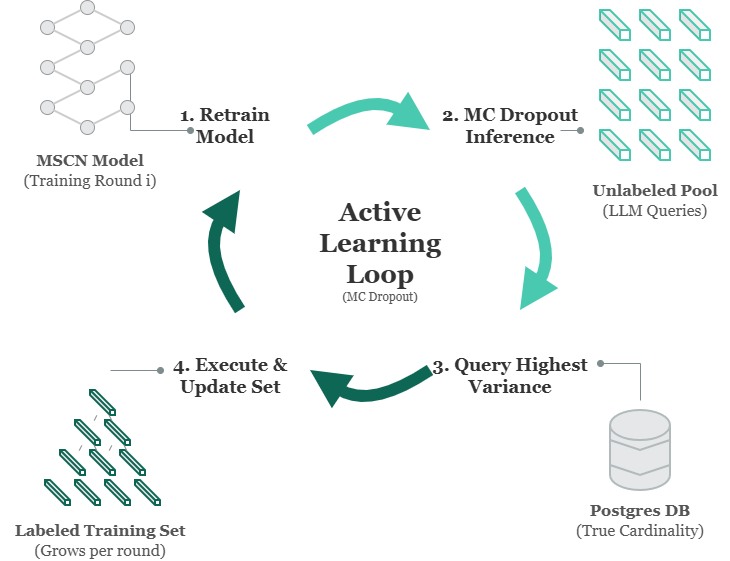
\includegraphics[width=0.85\linewidth, height=6.3cm, keepaspectratio]{active_leaning_diagram} 
		\end{center}
	\end{frame}
	
	% ==========================================
	\section{Experimental Results}
	
	% --- Slide 10: Setup + Validation ---
	\begin{frame}{Experimental Setup \& Data Quality}
		\small
		\begin{columns}[T]
			\column{0.45\textwidth}
			\textbf{Configuration:}
			\begin{itemize}
				\item \textbf{Database:} IMDB benchmark
				\item \textbf{LLM:} Llama 3.2 via Ollama
				\item \textbf{Model:} MSCN (hidden=256, dropout=0.1)
				\item \textbf{AL:} MC Dropout, $T=25$, 5 rounds
				\item \textbf{Metric:} Q-error
			\end{itemize}
			
			\column{0.55\textwidth}
			\begin{center}
				
\includegraphics[width=0.9\linewidth, height=5.0cm, keepaspectratio]{data_query_validation}
				
				\vspace{0.1cm}
				\scriptsize \textit{Query validation success rate across generation batches}
			\end{center}
		\end{columns}
	\end{frame}
	
	% --- Slide 11: Structural Diversity ---
	\begin{frame}{Workload Diversity}
		\vspace{-0.5cm}
		\begin{columns}
			\column{0.5\textwidth}
			\begin{center}
				
\includegraphics[width=\linewidth, keepaspectratio]{data_structural_features}
				
				\scriptsize \textit{Structural feature distributions}
			\end{center}
			
			\column{0.5\textwidth}
			\begin{center}
				
\includegraphics[width=\linewidth, keepaspectratio]{data_joins_distribution}
				
				\scriptsize \textit{Join count distribution}
			\end{center}
		\end{columns}
		
		\vspace{0.1cm}
		\begin{center}
			\scriptsize Diversity hints produce a balanced mix of single-table, two-table, and three-table queries with varied predicate counts.
		\end{center}
	\end{frame}
	
	% --- Slide 12: Cardinality Distribution ---
	\begin{frame}{Cardinality \& Predicate Coverage}
		\vspace{-0.5cm}
		\begin{columns}
			\column{0.5\textwidth}
			\begin{center}
				
\includegraphics[width=\linewidth, keepaspectratio]{data_cardinality_distribution}
				
				\scriptsize \textit{True cardinality distribution (log scale)}
			\end{center}
			
			\column{0.5\textwidth}
			\begin{center}
				
\includegraphics[width=\linewidth, keepaspectratio]{data_predicates_distribution}
				
				\scriptsize \textit{Predicate count distribution}
			\end{center}
		\end{columns}
		
		\vspace{0.1cm}
		\begin{center}
			\scriptsize Generated workload spans cardinalities from single-digit to millions, covering the full range needed for robust estimation.
		\end{center}
	\end{frame}
	
	% --- Slide 13: Q-error Results ---
	\begin{frame}{Estimation Accuracy: Q-error Analysis}
		\begin{columns}
			\column{0.5\textwidth}
			\begin{center}
				
\includegraphics[width=\linewidth, keepaspectratio]{test_qerror_cdf}
				
				\scriptsize \textit{Q-error CDF: majority within factor of 2--5}
			\end{center}
			
			\column{0.5\textwidth}
			\begin{center}
				
\includegraphics[width=\linewidth, keepaspectratio]{test_qerror_stats}
				
				\scriptsize \textit{Q-error statistics per AL round}
			\end{center}
		\end{columns}
		
		\vspace{0.2cm}
		\begin{center}
			\scriptsize Median, mean, and tail Q-errors all decrease with each active learning round.
		\end{center}
	\end{frame}
	
	% --- Slide 14: Labeling Efficiency ---
	\begin{frame}{Active Learning: Labeling Efficiency}
		\vspace{-0.5cm}
		\begin{columns}
			\column{0.5\textwidth}
			\begin{center}
				
\includegraphics[width=\linewidth, height=5.5cm, keepaspectratio]{analysis_labeling_efficiency}
				
				\scriptsize \textit{AL achieves competitive accuracy with fewer labels}
			\end{center}
			
			\column{0.5\textwidth}
			\begin{center}
				
\includegraphics[width=\linewidth, height=5.5cm, keepaspectratio]{train_learning_curve_random}
				
				\scriptsize \textit{Learning curve across AL rounds}
			\end{center}
		\end{columns}
		
		\vspace{0.1cm}
		\begin{center}
			\scriptsize Intelligent query selection reduces labeling cost by $\sim$40\% while maintaining estimation quality.
		\end{center}
	\end{frame}
	
	% --- Slide 15: PostgreSQL Comparison ---
	\begin{frame}{MSCN vs.\ PostgreSQL Optimizer}
		\vspace{-0.5cm}
		\begin{columns}
			\column{0.5\textwidth}
			\begin{center}
				
\includegraphics[width=\linewidth, height=5.5cm, keepaspectratio]{compare_pg_vs_mscn_cdf}
				
				\scriptsize \textit{Q-error CDF: MSCN vs. PostgreSQL}
			\end{center}
			
			\column{0.5\textwidth}
			\begin{center}
				
\includegraphics[width=\linewidth, height=5.5cm, keepaspectratio]{compare_pg_vs_mscn_scatter}
				
				\scriptsize \textit{Predicted vs. actual: closer to diagonal = better}
			\end{center}
		\end{columns}
		
		\vspace{0.1cm}
		\begin{center}
			\scriptsize The MSCN model trained with active learning matches or outperforms PostgreSQL's built-in estimator.
		\end{center}
	\end{frame}
	
	% ==========================================
	\section{Conclusion}
	
	% --- Slide 16: Conclusion ---
	\begin{frame}{Conclusion}
		\textbf{What we showed:}
		\begin{itemize}
			\item LLMs generate diverse, realistic SQL workloads from schema alone ($\sim$95\% valid)
			\item Active learning with MC Dropout reduces labeling cost by $\sim$40\%
			\item The trained MSCN matches PostgreSQL's built-in estimator
			\item The pipeline is schema-agnostic and fully automated
		\end{itemize}
		
		\vspace{0.5cm}
		
		\textbf{Future Directions:}
		\begin{itemize}
			\item Extend to richer SQL fragments (OR, LIKE, GROUP BY)
			\item Cross-schema transfer learning
			\item Integration with live query optimizers
			\item Hybrid acquisition: uncertainty + diversity
		\end{itemize}
	\end{frame}
	
	% ==========================================
	\section{References}
	
	% --- Slide 17: References ---
	\begin{frame}[allowframebreaks]{References}
		\begin{thebibliography}{9}
			\bibitem{kipf2018}
			Kipf, A., Kipf, T., Radke, B., Leis, V., Boncz, P., \& Kemper, A. (2019).
			\newblock Learned Cardinalities: Estimating Correlated Joins with Deep Learning.
			\newblock \emph{CIDR 2019}.
			
			\bibitem{wang2021}
			Wang, X., Qu, C., Wu, W., Wang, J., \& Zhou, Q. (2021).
			\newblock Are We Ready For Learned Cardinality Estimation?
			\newblock \emph{Proc. VLDB Endow.}, 14(9), 1640--1654.
			
			\bibitem{davitkova2025}
			Davitkova, A. \& Michel, S. (2025).
			\newblock Automated Training of Learned Database Components with Generative AI.
			\newblock \emph{CoRR}, abs/2512.20271.
			
			\bibitem{gal2016}
			Gal, Y. \& Ghahramani, Z. (2016).
			\newblock Dropout as a Bayesian Approximation.
			\newblock \emph{ICML 2016}, 1050--1059.
		\end{thebibliography}
	\end{frame}
	
	% --- Slide 18: Thank You ---
	\begin{frame}[plain]
		\centering
		\Huge \textbf{Thank you}
		
		\vspace{1cm}
		\normalsize
		\textbf{Preksha Shah} \\
		qar12xun@rptu.de \\
		RPTU Kaiserslautern
	\end{frame}
	
\end{document}